\documentclass[]{article}
\usepackage[utf8]{inputenc}
\usepackage[margin=1in]{geometry}
\usepackage{graphicx}
\usepackage{amsmath,amscd}
\usepackage{graphics} % for pdf, bitmapped graphics files
\usepackage{epsfig} % for postscript graphics files
\usepackage{mathptmx} % assumes new font selection scheme installed
\usepackage{times} % assumes new font selection scheme installed
\usepackage{amssymb}  % assumes amsmath package installed
\usepackage{multirow}
\usepackage{cite}
\usepackage{subfigure}
\usepackage{booktabs}

\newcommand{\beqa}{ \begin{eqnarray}}
\newcommand{\eeqa}{ \end{eqnarray} }
\newcommand{\beq}{ \begin{equation}}
\newcommand{\eeq}{ \end{equation} }
\newcommand{\baa}{ \left(\begin{array}}
\newcommand{\eaa}{ \end{array}\right) }
\newcommand{\IR}{\mathbb{R}}
\newcommand{\II}{\mathbb{I}}
\newcommand{\tr}{\mbox{tr}}
\newcommand{\OO}{{\bf O}}
\newcommand{\xx}{{\bf X}}
\newcommand{\nn}{{\bf n}}
\newcommand{\epa}{{\epsilon_1}}
\newcommand{\epb}{{\epsilon_2}}
\newcommand{\ttt}{{\bf t}}

\title{Closed-form Minkowski Sum/Difference between Ellipsoid and Superquadrics}

\begin{document}

\maketitle

\section{Mathematical Preliminaries} \label{mathsec}

In this section, the basics of Minkowski sums are reviewed.
The Minkowski sum of two convex point sets (or bodies) each centered at the origin, $P_1$ and $P_2$ in $\cal R^n$, is defined as
\begin{equation} \label{minksundef}
P_1 \oplus P_2 \,\doteq\, \{p_1+p_2~|~p_1 \in P_1, p_2 \in P_2 \}
\end{equation}
The Minkowski difference between $P_1$ and $P_2$ is defined as \cite{chiu2013stochastic}
\begin{equation}
P_1 \ominus P_2 \,\doteq\, \bigcap_{p_2 \in P_2} (P_1+p_2)
\end{equation}
Alternatively, the Minkowski difference of two convex bodies can be defined relative
to the Minkowski sum as the body $P'_1 = P_1 \ominus P_2$ for which
$P_1 = P'_1 \oplus P_2$.

Minkowski operations are used in a wide range of applications such as robot motion planning \cite{latombe1991robot}, CAD/CAM, assembly planning \cite{halperin2000general} and computer-aided design \cite{hartquist1999computing}. For example, consider an obstacle $P_1$ and a robot $P_2$ that moves by translation. By choosing a reference point attached to $P_2$, then $P_1 \oplus P_2$ is the locus of positions of the reference point where $P_1 \cap P_2 \neq \emptyset$. In the study of motion planning this sum is called a C-space obstacle. Alternatively, if $P_1$ is an ``arena'' (i.e., a bounded workspace) in which the robot $P_2$ is moving, then $P_1 \ominus P_2$ is the locus of positions of the reference point where $P_1 \cap P_2 = P_2$, and represents the robot's collision-free C-space with respect to the arena. While defining the Minkowski operations mathematically is easy, computing useful representations of Minkowski sums or differences can be difficult and computationally expensive, especially when the exact boundary of the geometry of these entries need to be represented explicitly. Many algorithms exist for numerically computing the boundary of the Minkowski sum of polygonal/polyhedral sets in two/three dimensions \cite{guibas1983kinetic,fogel2007exact,hachenberger2009exact,agarwal2002polygon,behar2011dynamic,hartquist1999computing}. These algorithms mainly either compute the convolution of geometric boundaries \cite{guibas1983kinetic}, or use polygon/polyhedra decompositions \cite{agarwal2002polygon,fogel2007exact,hachenberger2009exact,hartquist1999computing}. Minkowski sums of curved regions/surfaces have also been studied (e.g. \cite{bajaj1989generation,sack1999handbook,kaul1995computing,lee1998polynomial}).

\section{Closed-form Minkowski Operations Between an Ellipsoid and a Superquadric} \label{mink-es}
In this section, the closed-form Minkowski operations between an ellipsoid and a superquadric are introduced. The derivation applies a combination of affine transformations and the analytic properties of offset surfaces. The calculations in both 2-dimensional (ellipse-superellipse) and 3-dimensional (ellipsoid-superquadric) cases are provided. The resulting characterizations describe an exact lower or upper boundary of an ellipsoid and a superquadric by using Minkowski sum or difference operation respectively, after which a collision-free area of the two objects can be decided.

The results of this section form the basic building blocks to describe C-space obstacles, and are used
in Section IV to sample from the collision-free C-space of poly-ellipsoidal humanoid figures and multiple
superquadric obstacles.

\subsection{Closed-form Minkowski Operations Between an Ellipse and a Superellipse}
The implicit equation for a superellipse $SQ_1$ in a 2-dimensional Euclidean space is defined as

\begin{equation}
\left(\dfrac{x_1}{a_1} \right)^{\frac{2}{\epsilon}} + \left( \dfrac{y_1}{b_1}\right)^{\frac{2}{\epsilon}} = 1
\label{2dsq}
\end{equation}
And the corresponding explicit equation can then be written as:
\begin{equation}
{\bf x}_1 = \left(
\begin{array}{c}
x_1 \\ y_1
\end{array}
\right)
=
\left(
\begin{array}{c}
a_1 \cos^{\epsilon}\theta \\
b_1 \sin^{\epsilon}\theta
\end{array}
\right)
, \; \;
-\pi \leq \theta \leq \pi
\label{sq2de}
\end{equation}
The exponentiation with $\epsilon$ is a signed power function such that $\cos^{\epsilon}\theta = \text{sign}(\cos\theta)|\cos\theta|^{\epsilon}$. The shape described by the above function can change with $\epsilon$, and we only consider the case of $0 < \epsilon < 2$ so that the corresponding shape will always be convex.

With the above knowledge of superellipse, we define a superelliptic surface as:
\begin{equation}
F(x_1, y_1) = \left(\dfrac{x_1}{a_1} \right)^{\frac{2}{\epsilon}} + \left( \dfrac{y_1}{b_1}\right)^{\frac{2}{\epsilon}} - 1
\end{equation}
Then the normal vector of the superellipse can be obtained by calculating the gradient of $F(x_1, y_1)$:

\begin{equation}
\nabla F(x_1,y_1) =
\left[ \dfrac{2}{a_1 \epsilon}\left(\dfrac{x_1}{a_1} \right)^{\frac{2}{\epsilon } - 1}, \dfrac{2}{b_1\epsilon}\left(\dfrac{y_1}{b_1} \right)^{\frac{2}{\epsilon} - 1} \right]^{T}
\label{sq2dg}
\end{equation}
Substituting Eq.\eqref{sq2de} into Eq.\eqref{sq2dg} and normalizing the obtained parametric gradient gives a unit normal vector of the superellipse:
\begin{equation}
\nabla F(x_1(\theta), y_1(\theta)) = \dfrac{2}{\epsilon}
\left(
\begin{array}{c}
\cos^{2 - \epsilon}\theta /a_1 \\
\sin^{2 - \epsilon}\theta /b_1
\end{array}
\right)
\end{equation}

\begin{equation}
{\bf n}(\theta) =
\dfrac{\nabla F}{||\nabla F||} \; \; \text{where} \; \; 0 < \epsilon < 2
\end{equation}
%Note that when $\epsilon < 1$, ${\bf t}(\theta)$  and ${\bf n}(\theta)$ are not defined at $\theta = n\pi/2$ where $n = 0,1,2 \dots$. When $\epsilon > 1$, ${\bf t}(\theta) \equiv \bf 0 $  and ${\bf n}(\theta) \equiv \bf 0 $ for $\theta = n\pi/2$ where $n = 0,1,2 \dots$.

%The tangent vector is defined as:
%\begin{equation}
%{\bf \mathbb{T}}(\theta)
%=
%\left(
%\begin{array}{c}
%- a_1\epsilon \sin\theta \cos^{\epsilon -1}\theta\\
%b_1\epsilon \cos\theta \sin^{\epsilon - 1}\theta
%\end{array}
%\right)
%\end{equation}
%
%The normal outward-pointing vector is defined as:
%\begin{equation}
%{\bf \mathbb{N}}(\theta) =
%\left(
%\begin{array}{c}
%b_1\epsilon \cos\theta \sin^{\epsilon - 1}\theta\\
%a_1\epsilon \sin\theta \cos^{\epsilon -1}\theta
%\end{array}
%\right)
%\end{equation}
The rotated version of the superellipse where the principal axes are oriented by rotation matrix $R_1$ relative to the world reference frame is:
\begin{equation}
{\bf x}_{1r}  = R_1 {\bf x}_1
\end{equation}

\begin{figure}[!t]
	\centering
	\subfigure[Both bodies are rotated clockwise with an angle $\theta_2$.]{
		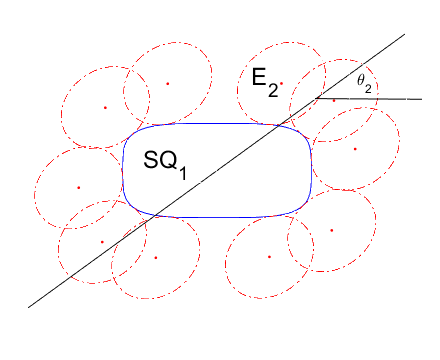
\includegraphics[scale=0.3]{ES_sum_1.png}}
	\hspace{0.1in}
	\subfigure[Both of the bodies are shrunk until $\partial E_2$ becomes a circle.]{
		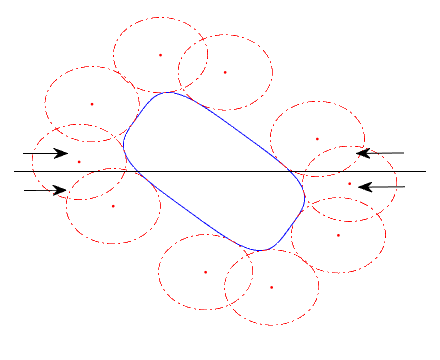
\includegraphics[scale=0.3]{ES_sum_2.png}}
	\\
	\subfigure[The Minkowski sum in this transformed space is an offset surface (the shaded area).]{
		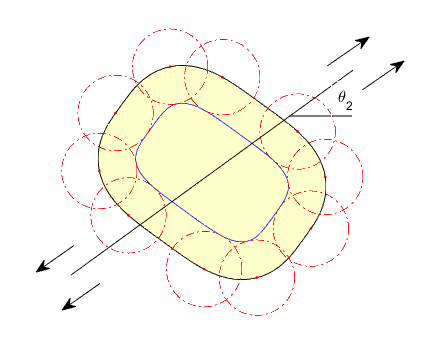
\includegraphics[scale=0.3]{ES_sum_3.png}}
	\hspace{0.1in}
	\subfigure[Everything is then stretched and rotated back until the surrounding circle in \textbf{c} becomes the original version of $\partial E_2$ again. The shaded region represents $SQ_1 \oplus E_2$.]{
		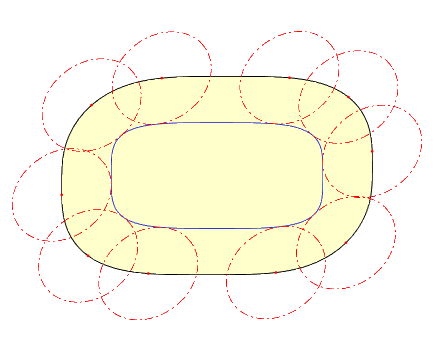
\includegraphics[scale=0.3]{ES_sum_complete.png}}
	\caption{Algorithm for obtaining the parametric representation of the boundary of the Minkowski sum of a superelliptical body $SQ_1$ and an ellipse body $E_2$.}
	\label{fig:M-sum}
\end{figure}

Given a rotated ellipse $E_2$ defined by the implicit equation:
\begin{equation}
{\bf x}_2^{T}R_2\Lambda^{-2}({\bf a}_2)R_2^{T}{\bf x}_2 = 1
\end{equation}
where $R_2 \in SO(2)$, ${\bf x}_2 = \left[x_2, y_2\right]^T$, ${\bf a}_2 = \left[a_2, b_2\right]$ and $\Lambda({\bf a}_2) = diag(a_2, b_2) \in \mathbb{R}^{2 \times 2}$. If we further define $r = \text{min}(a_2, b_2)$, then the transformation defined as $T_s = R_2\Lambda^{-1}({\bf a}_2/r)R_2^{T}$ on ${\bf x}_2$ will transform $E_2$ into a 2 dimensional sphere.
The corresponding ``shrinking'' version of the superellipse is
\begin{equation}
{\bf x}_1^{\prime}  = T_s {\bf x}_{1r} = T_s R_1{\bf x}_{1} = T_r {\bf x}_{1}
\label{shrinkrotsq}
\end{equation}
Now, for the normal vector of the shrunk and rotated superellipse, we define $T_r$ to be:
\begin{equation}
T_r^{-1} =
\left(
\begin{array}{lr}
t_{11} & t_{12} \\
t_{21} & t_{22}
\end{array}
\right)
\end{equation}

Then according to Eq.\eqref{shrinkrotsq},
\begin{equation}
\left(
\begin{array}{c}
x_1 \\
y_1
\end{array}
\right)
=
{\bf x}_1
=
T_r^{-1}{\bf x}_1^{\prime}
=
\left(
\begin{array}{c}
t_{11}x_1^{\prime} + t_{12}y_1^{\prime} \\
t_{21}x_1^{\prime} + t_{22}y_1^{\prime}
\end{array}
\right)
\label{invsq}
\end{equation}
Substitute Eq.\eqref{invsq} back into Eq.\eqref{2dsq} and calculate the gradient of $F(x_1^{\prime}, y_1^{\prime})$ with respect to $x_1$ and $y_1$:
\begin{equation}
\nabla F^{\prime}(x_1^{\prime}, y_1^{\prime}) =
\left(
\begin{array}{lr}
t_{11} & t_{21} \\
t_{12} & t_{22}
\end{array}
\right)
\left(
\begin{array}{c}
\dfrac{2}{a_1\epsilon}
\left( \left( t_{11} x_1^{\prime} + t_{12} y_1^{\prime} \right) /a_1 \right)^{2/\epsilon - 1} \\
\dfrac{2}{b_1\epsilon}
\left(\left( t_{21} x_1^{\prime} + t_{22} y_1^{\prime} \right) /b_1 \right)^{2/\epsilon - 1}
\end{array}
\right)
\label{trangradient}
\end{equation}
Substitute Eq.\eqref{invsq} into Eq.\eqref{trangradient} and normalize the gradient, we get the unit normal vector:
\begin{equation}
\nabla F^{\prime}(x_1^{\prime}(x_1), y_1^{\prime}(y_1) ) = T_r^{-T}
\left(
\begin{array}{c}
\dfrac{2}{a_1\epsilon}
\left(x_1 /a_1 \right)^{2/\epsilon - 1} \\
\dfrac{2}{b_1\epsilon}
\left(y_1 /b_1 \right)^{2/\epsilon - 1}
\end{array}
\right)
\end{equation}

\begin{equation}
\nabla F^{\prime}(x_1^{\prime}(\theta), y_1^{\prime}(\theta) ) = T_r^{-T}
\nabla F(x_1(\theta), y_1(\theta))
\end{equation}

\begin{equation}
{\bf n}^{\prime}(\theta) =
\dfrac{\nabla F^{\prime}}{||\nabla F^{\prime}||} \; \; \text{where} \; \; 0 < \epsilon < 2
\end{equation}

\begin{figure}[!t]
	\centering
	\subfigure[]{
		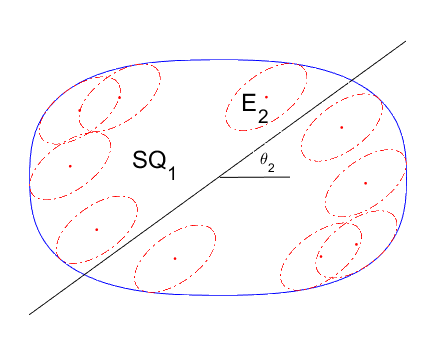
\includegraphics[scale=0.3]{ES_diff_1.png}}
	\hspace{0.1in}
	\subfigure[]{
		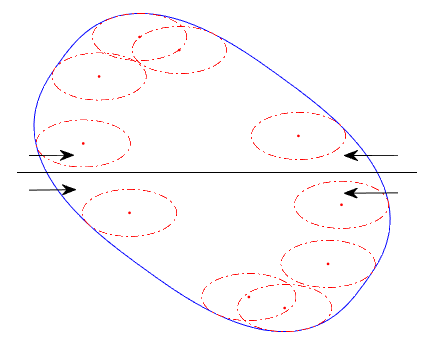
\includegraphics[scale=0.3]{ES_diff_2.png}}
	\\
	\subfigure[]{
		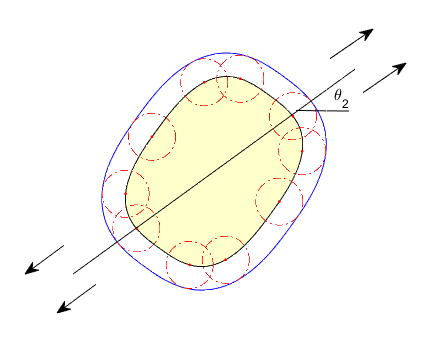
\includegraphics[scale=0.3]{ES_diff_3.png}}
	\hspace{0.1in}
	\subfigure[]{
		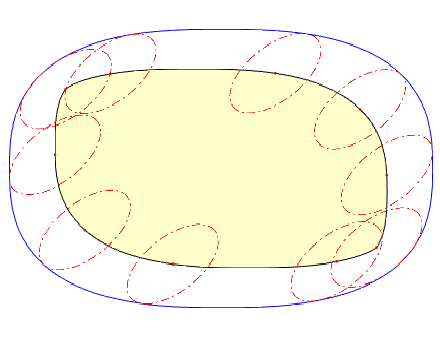
\includegraphics[scale=0.3]{ES_diff_complete.png}}
	\caption{Algorithm for obtaining the parametric representation of the boundary of the Minkowski difference of a superelliptical body $SQ_1$ and an elliptical body $E_2$. This presumes that the radius of curvature of the rotated and shrunk ellipse ($E_2$), which becomes a circle, is smaller than that of the bounding rotated and shrunk superellipse at every point. The algorithm follows the same steps as Figure \ref{fig:M-sum}. The shaded region represents $SQ_1 \ominus E_2$}
	\label{fig:M-diff}
\end{figure}

A parametrized offset hyper-surface ${\bf x}_{fos}(\theta)$ of an orientable, closed and differentiable hyper-surface ${\bf x}(\phi) \in \mathbb{R}$ with the offset radius $r = min\{a_1, a_2, \dots, a_n\}$ is defined as:
\begin{equation}
{\bf x}_{ofs}(\phi) = {\bf x}(\phi) + r{\bf n}(\phi)
\end{equation}
For the case of a superellipse and an ellipse,
\begin{equation}
{\bf x}_{1ofs}^{\prime}(\theta) = {\bf x}_1^{\prime}(\theta) + r{\bf n}^{\prime}(\theta)
\label{sumoffset}
\end{equation}
Then the exact boundary of the Minkowski sum of $SQ_1 \oplus E_2$ can be represented in closed-form as:
\begin{equation}
{\bf x}_{eb} = T_s^{-1}{\bf x}_{1ofs}^{\prime}(\theta)
\end{equation}

The Minkowski difference $SQ_1 \ominus E_2$ has similar expression except that Eq.\eqref{sumoffset} will have minus sign to calculate the inward offset curve. Note that for Minkowski difference, it is not always possible to subtract an ellipse from a superellipse. It can only be done if after applying the affine transformation that converts the ellipse to a circle, that the minimal radius of curvature of the transformed superellipse is greater than the radius of the circle that the ellipse transformed into. This condition is necessary because otherwise the ellipse will not fit inside a superellipse and kiss the boundary without overlapping. 

Concretely, the curvature of the transformed superellipse can be derived from the implicit expression of the curve as follows.
\begin{equation}
m = \frac{\| \nabla F' \|^2 \tr(\nabla \nabla^T F') - (\nabla^T F')(\nabla \nabla^T F')(\nabla F')}{2 \| \nabla F' \|^3} = \nabla \cdot (\frac{\nabla F'}{\| \nabla F \|})
\end{equation}

An illustration of Minkowski operation on ellipses and superquadrics can be seen as in Fig.~\ref{fig:M-sum} and Fig.~\ref{fig:M-diff}.

\subsection{Closed-form Minkowski Operations Between an Ellipsoid and a Superquadrics}
We now briefly show that the same closed-form Minkowski operations can be extended to the 3D case. The implicit equation for superquadrics is:
\begin{equation}
\left( \left( \dfrac{x}{a} \right)^{\frac{2}{\epb}} +
\left( \dfrac{y}{b}\right)^{\frac{2}{\epb}}
\right)^{\frac{\epsilon_2}{\epsilon_1}}
+
\left( \dfrac{z}{c}\right)^{\frac{2}{\epsilon_1}} = 1
\label{superquadrics}
\end{equation}
The corresponding explicit equation is:
\begin{equation}
{\bf x} =
\left(
\begin{array}{c}
x \\
y \\
z
\end{array}
\right)
=
\left(
\begin{array}{c}
a\cos^{\epsilon_1} \eta \cos^{\epsilon_2} \omega \\
b\cos^{\epsilon_1} \eta \sin^{\epsilon_2} \omega \\
c\sin^{\epsilon_1} \eta
\end{array}
\right)
,
\begin{array}{c}
-\pi/2 \leq \eta \leq \pi/2 \\
- \pi \leq \omega < \pi
\end{array}
\end{equation}
The normal vector a point $(x,y,z)(\eta, \omega)$ on the superellipsoid surface is defined as:
\begin{equation}
\begin{split}
& \mathbb{N}_1(\eta, \omega) = {\bf r}_{\eta}(\eta, \omega) \times {\bf r}_{\omega}(\eta, \omega) \\
=&\left(
\begin{array}{c}
-bc \epa \epb\sin^{\epa - 1}\eta \cos^{\epa + 1}\eta \cos\omega\sin^{\epb - 1}\omega\\
-ac \epa \epb\sin^{\epa - 1}\eta \cos^{\epa + 1}\eta \sin\omega\cos^{\epb - 1}\omega\\
-ab \epa \epb\sin\eta \cos^{2\epa - 1}\eta \sin^{\epb - 1}\omega\cos^{\epb - 1}\omega
\end{array}
\right) \\
=& f(\eta, \omega) \mathbb{N}_2(\eta, \omega)
\end{split}
\end{equation}
where\
\begin{equation}
{\bf r}_{\eta}(\eta, \omega) =
\left(
\begin{array}{c}
-a\epsilon_1\sin\eta\cos^{\epsilon_1-1}\eta\cos^{\epsilon_2}\omega\\
-b\epsilon_1\sin\eta\cos^{\epsilon_1-1}\eta\sin^{\epsilon_2}\omega\\
c{\epsilon_1}\sin^{\epsilon_1 - 1}\cos{\eta}
\end{array}
\right)
\end{equation}
and
\begin{equation}
{\bf r}_{\omega}(\eta, \omega) =
\left(
\begin{array}{c}
-a\epsilon_2\cos^{\epsilon_1}\eta\sin\omega\cos^{\epsilon_2 - 1}\omega\\
b\epsilon_2\sin\eta\cos^{\epsilon_1}\eta\cos\omega\sin^{\epsilon_2 - 1}\omega\\
0
\end{array}
\right)
\end{equation}
${\bf r}_{\eta}(\eta, \omega)$ and ${\bf r}_{\omega}(\eta, \omega)$ are tangent vectors along $\eta$ and $\omega$ respectively.

After extracting and dropping a common factor of $\nn(\eta, \theta)$, an equivalent form of normal vector can be obtained as:
\begin{equation}
\nabla F(x, y, z) =  \mathbb{N}_2(\eta, \omega) =
\left(
\begin{array}{c}
\cos^{2 - \epa}\eta \cos^{2-\epb}\omega /a \\
\cos^{2 - \epa}\eta \sin^{2-\epb}\omega /b \\
\sin^{2-\epb}\eta /c
\end{array}
\right)
\end{equation}
The corresponding normalized normal vector will be:
\begin{equation}
\nn(\eta, \theta) = \dfrac{\mathbb{N}_2 (\eta, \omega)}{||\mathbb{N}_2 (\eta, \omega)||}
\end{equation}
For the case where $\epsilon_1 = \epsilon_2 = \epsilon$,  Eq~.(\ref{superquadrics}) will become:
\begin{equation}
\left( \dfrac{x}{a} \right)^{\frac{2}{\epsilon}} +
\left( \dfrac{y}{b}\right)^{\frac{2}{\epsilon}}
+
\left( \dfrac{z}{c}\right)^{\frac{2}{\epsilon}} = 1
\label{superellipsoid}
\end{equation}
The explicit equation is:
\begin{equation}
{\bf x} =
\left(
\begin{array}{c}
x \\
y \\
z
\end{array}
\right)
=
\left(
\begin{array}{c}
a\cos^{\epsilon} \eta \cos^{\epsilon} \omega \\
b\cos^{\epsilon} \eta \sin^{\epsilon} \omega \\
c\sin^{\epsilon} \eta
\end{array}
\right)
,
\begin{array}{c}
-\pi/2 \leq \eta \leq \pi/2 \\
- \pi \leq \omega < \pi
\end{array}
\end{equation}
If we further define a transformation $T-r = R_2 \Lambda^{-2}({\bf a}_2/r)R_2^{T}R_1$ on $\bf x$ such that ${\bf x}^{'} = T_r {\bf x}$, it follows as in the 2D case that $\nabla^{\prime}F = T_r^{-T} \nabla F$. The offset surfaces of the Minkowski sum $SQ_1 \oplus E_2$ and difference $SQ_1 \ominus E_2$ follow the same fashions as in the 2D case. In terms of Minkowski difference, the discussion of the possibility to obtain a valid result is the same as in the 2D case; instead, ellipses, circles and superellipses become ellipsoids, spheres and superquadrics respectively.

\end{document}
